% Scientific appendix. Full numerical records and supplementary derivations are packaged separately.
\section{Proofs, identification, and calibration}
\label{app:proofs}
\subsection{Fixed row coverage and exposure-weighted coverage}
% Show the moved Proposition 1 without disturbing subsequent numbering.
\begingroup
\renewcommand{\theproposition}{1}
\renewcommand{\theHproposition}{threshold}
\begin{proposition}[Fixed-coverage threshold principle]
\label{prop:threshold}
Assume $\E|L-rW|<\infty$. Among rules with $\E a=c$, accepting
the smallest $m_r=\E[L-rW\mid X]$ values minimizes expected excess.
Boundary randomization resolves atoms. The minimum excess is
$\int_0^cQ_m(u)\,du$, where $Q_m$ is the quantile function of $m_r$.
A ratio-risk assertion additionally requires positive accepted exposure.
\end{proposition}
\endgroup
\addtocounter{proposition}{-1}
Choose $t$ with $\Pr(m_r<t)\leq c\leq\Pr(m_r\leq t)$, and let
$a^*$ accept below $t$, reject above it, and randomize on the tie
to attain $c$. For any other rule of the same coverage,
\[
 (a-a^*)(m_r-t)\geq0,\qquad
 \E[a(L-rW)]-\E[a^*(L-rW)]
 =\E[(a-a^*)(m_r-t)]\geq0.
\]
This proves the threshold rule and the lower-quantile expression.
The limiting rules cover $c=0,1$. This minimizes excess, not the
ratio itself at fixed row coverage, because accepted exposure can vary.

For Proposition~\ref{prop:weighted}, $w=0$ implies $W=0$ almost
surely conditionally. These contexts add no exposure: reject them
if $\ell>0$; otherwise they are neutral. On $\{w>0\}$, set
$d\nu=w\,dP_X/T$ and $\xi=\ell/w$. Then
\[
 \E[aW]=T\E_\nu a,\qquad \E[aL]=T\E_\nu[a\xi].
\]
The exchange argument under $\nu$ minimizes the numerator at fixed
exposure coverage by ordering $\xi$. Maximizing feasible exposure
coverage thus admits an $\ell/w$ threshold when a positive-exposure
feasible rule exists. An additional binding row floor can change
that optimizer. Randomization handles atoms; the ranking is
independent of $r$, while the selected threshold depends on $r$.

% Replaces review4_theory_proofs.tex; Appendix A.1 uses generic ell,w.
\subsection{Sharp reversal for nonnegative ratio risks}
\paragraph{Proof of Proposition~\ref{prop:lowdemand}.}
Since $\ell=\rho w$ on $U$, its error-to-exposure ratio is $\rho$
and its excess mass is $(\rho-r)M_U$. The combined excess is
$-B+(\rho-r)M_U$, proving the first assertion and the coverage increments.

For sharpness, take $k,p,q>0$ with $k+p+q=1$, $k>c_0$, $q>p$,
and $0<\varepsilon<p/q$. Set the conditional moments to
\[
\begin{array}{c|ccc}
 &K&U&V\\\hline
 \Pr(X)&k&q&p\\
 w&\dfrac{q(\rho-r)\varepsilon}{rk}&\varepsilon&1\\
 \ell&0&\rho\varepsilon&r+\dfrac qp(\rho-r)\varepsilon
\end{array}
\]
They can be realized simply by deterministic $(L,W)=(\ell,w)$.
Their excesses are
\[
 m_K=-\frac{q(\rho-r)\varepsilon}{k},\quad
 m_U=(\rho-r)\varepsilon,\quad
 m_V=\frac qp(\rho-r)\varepsilon.
\]
Every optimum accepts $K$, since doing so increases either utility
and relaxes the constraint. Its budget is $B=q(\rho-r)\varepsilon$.
Once $K$ is accepted, feasibility reduces to $a_U+a_V\leq1$.
Row utility is maximized uniquely at $(a_U,a_V)=(1,0)$ since $q>p$;
exposure utility is maximized uniquely at $(0,1)$ since $q\varepsilon<p$.
These arguments optimize over all fractional acceptance rules.
Both policies have ratio risk $r$ and row coverage above $c_0$.
With $T=p+q\rho\varepsilon/r$,
\[
 \Delta c=q-p,\qquad
 d_W(a_R)=\frac{q\rho\varepsilon}{rp+q\rho\varepsilon},\qquad
 \Delta d_W=\frac{r(p-q\varepsilon)}{rp+q\rho\varepsilon}.
\]
Take $k>c_0$ sufficiently near $c_0$ and then $p>0$ sufficiently
small that $q-p=1-k-2p>1-c_0-\eta$; for these masses,
$\varepsilon\downarrow0$ gives $\Delta d_W\to1$.
The opposite inequalities follow from $c(a_R)\leq1$,
$c(a_W)\geq c_0$, and $0\leq d_W\leq1$.

For $0<r<1$, choose $\rho=1$ and scale all moments by
$h=1/\max(1,w_K)$, which leaves risks, both coverages, and both
optimizers unchanged. Then $0\leq\ell\leq w\leq1$.
At each context, put probabilities $\ell,w-\ell,1-w$ on
$(L,W)=(1,1),(0,1),(0,0)$. This realizes the same conditional moments
with nested binary events, proving bounded-loss sharpness.
For the deterministic WAPE specialization before scaling, take
$Y=(w_K,\varepsilon,1)$ and
$f=(w_K,0,(1-r)(1-q\varepsilon/p))$. These nonnegative forecasts
realize precisely the $\rho=1$ moments. \hfill$\square$

\paragraph{Scope of the realizability condition.}
The displayed moment family is a sufficient condition for a fixed
loss/exposure model class to inherit the sharp bounds. In this
three-context family the strict inequalities $q>p$ and
$q\varepsilon<p$ are also necessary for these two distinct, unique
optima. They are not necessary conditions for reversal in arbitrary
larger classes. Ratio form, nonnegativity, and integrability alone
do not make every specified metric class rich enough: constant
$w$ makes exposure and row utility proportional. For a precision-like
error ratio, $L=\ind\{\widehat Y=1,Y=0\}$ and
$W=\ind\{\widehat Y=1\}$; for a recall-like miss ratio,
$L=\ind\{Y=1,\widehat Y=0\}$ and $W=\ind\{Y=1\}$.
Both have $L\leq W$, but realization requires acceptance to be
chosen using information for which the joint event probabilities
can take the three specified values. A deterministic prediction
included in $X$ restricts these moments. Recall here is conditional
on accepted cases; a metric counting rejected positives in its
fixed denominator is a different constraint.

\paragraph{A margin-dependent bound.}
For alternatives $K\cup U$ and $K\cup V$, suppose $\ell=\rho w$
on $U$ and $U$ exhausts the common slack:
$B=(\rho-r)M_U>0$. If $K\cup V$ satisfies the cap, $M_V>0$,
and $R(\ind_V)-r\geq\delta>0$, then
\[
 d_W(\ind_{K\cup V})-d_W(\ind_{K\cup U})
 \leq\frac{M_U}{T}\left(\frac{\rho-r}{\delta}-1\right).
\]
Indeed, $\delta M_V\leq\E[\ind_Vm_r]\leq B$.
If both alternatives exhaust the same budget, the exact identity is
\[
 \Delta d_W=\frac{M_U}{T}
 \frac{\rho-R(\ind_V)}{R(\ind_V)-r}.
\]
The construction has $M_U/T\to0$ but $R(\ind_V)-r\to0$ as well;
this is why exposure share alone gives no vanishing bound.
For WAPE near-zero forecasts satisfy
$|\E[\ind_U e]-M_U|\leq\E[\ind_Uf]$, and hence
$|R(\ind_U)-1|\leq\E[\ind_Uf]/M_U$.

\paragraph{Finite perturbations of estimated rankings.}
Let $\widehat\ell=\ell+\delta_\ell$,
$\widehat w=w+\delta_w$, where $w>0$ and
$|\delta_w|\leq\beta w$ for some $0\leq\beta<1$. Direct subtraction gives
\[
 \left|\frac{\widehat\ell}{\widehat w}-\frac\ell w\right|
 =\frac{|w\delta_\ell-\ell\delta_w|}{w|w+\delta_w|}
 \leq\frac{|\delta_\ell|+(\ell/w)|\delta_w|}{(1-\beta)w}.
\]
In contrast, $|\widehat m_r-m_r|\leq|\delta_\ell|+r|\delta_w|$.
The local derivatives with respect to $w$ are $-\ell/w^2$ and $-r$;
the ratio's sensitivity with respect to $\ell$ is $1/w$.
These are sensitivity statements, not a proof that denominator
noise alone causes the observed empirical ordering.
For fixed $T>0$, write $b=(1-\lambda)/T$ and
$s_\lambda=(\ell-rw)/(\lambda+bw)$. When $0<\lambda\leq1$ and
$w,\widehat w\geq0$, the denominator is at least $\lambda$, and
\[
 \left|\widehat s_\lambda-s_\lambda\right|
 \leq\frac{|\delta_\ell|+r|\delta_w|}{\lambda}
 +\frac{|m_r|b|\delta_w|}{\lambda^2}.
\]
Its derivatives satisfy
\[
 \frac{\partial s_\lambda}{\partial w}
 =-\frac{r\lambda+b\ell}{(\lambda+bw)^2},\qquad
 \frac{\partial s_\lambda}{\partial\ell}
 =\frac{1}{\lambda+bw}\leq\frac1\lambda.
\]
Thus positive row utility removes the small-denominator singularity
for fixed bounded moments. It does not remove fitting error,
calibration error, or distribution shift. A floor $\max(\widehat w,c)$
likewise bounds denominator sensitivity, while changing the
unregularized population ranking.

% Fixed-classifier application; append to Appendix A.2.
\paragraph{Fixed classifiers: the unit of abstention matters.}\label{app:classification}
For ordinary binary precision, let $h(X)\in\{0,1\}$ be fixed,
$W=h(X)$, and $L=h(X)\ind\{Y=0\}$, with $T=\Pr(h(X)=1)>0$.
An unrestricted gate observing $h(X)$ cannot exhibit strict optimal
coverage reversal. Completing any feasible gate $a$ by accepting every
predicted-negative case leaves its risk and exposure unchanged and gives
\[
 a^+=(1-h)+ha,\qquad c(a^+)=1-T+T d_W(a).
\]
Whenever a positive-exposure feasible gate exists, $\sup c=1-T+T\sup d_W$: every row optimum is exposure-optimal,
and an exposure optimum can be completed to a row optimum.
This also holds with a common minimum row coverage.

A fixed \emph{multi-label} classifier with whole-example abstention does
exhibit reversal, because cases can contain different numbers of positive
predictions. Take two labels and three fully observed contexts:
\[
\begin{array}{c|ccc}
 &K&U&V\\\hline
 \Pr(X)&2/5&2/5&1/5\\
 h(X)&(1,0)&(1,0)&(1,1)\\
 w=\#\text{positive predictions}&1&1&2\\
 \ell=\E[\#\text{false positives}\mid X]&0&3/10&1/2
\end{array}
\]
At $K$, $Y=(1,0)$; at $U$, $Y=(0,0)$ with probability $3/10$
and $(1,0)$ otherwise; at $V$, $Y=(1,0)$ or $(1,1)$ equiprobably.
The gate observes all of $X$ and independently accepts the entire
prediction vector with probability $a(X)$.
The risk is one minus accepted micro-precision, with $r=1/10$ and
$c_0=7/20$. Every optimum accepts $K$; the remaining budget is
$4a_U+3a_V\leq2$. The unique row and exposure optima are
\[
\begin{array}{c|ccc}
 &a&(c,d_W)&R\\\hline
 \text{rows}&(1,1/2,0)&(3/5,1/2)&1/10\\
 \text{positive exposure}&(1,0,2/3)&(8/15,5/9)&1/10
\end{array}
\]
Hence $\Delta c=1/15$ and $\Delta d_W=1/18$.
Dividing both $L,W$ by two gives $0\leq L\leq W\leq1$ without
changing these results. Exact vertex enumeration and an independent LP
verify both optima. The example uses whole-case acceptance; independently
gating each label would define a different decision problem.

% Bounded positive-exposure geometry; insert after the fixed-classifier example.
\paragraph{Bounded exposure limits the reversal.}\label{app:bounded_exposure}
Suppose $0<u\leq w(X)\leq v<\infty$. For any row and exposure optima
under the same feasible set, put $x=c(a_R)-c(a_W)\geq0$,
$y=d_W(a_W)-d_W(a_R)\geq0$, and $D=(v-u)/(v+u)$. Then
\[
 y\leq\frac{D-x}{1-Dx},\qquad 0\leq x,y\leq D.
\]
To see this, let $b=\E(a_R-a_W)_+$ and $a=\E(a_W-a_R)_+$.
Then $b=a+x$, $a+b\leq1$, and bounding the positive and negative
exposure masses gives
$y\leq\{(v-u)a-ux\}/\{u+(v-u)a\}$, which increases with $a$.
Substitute $a\leq(1-x)/2$; a row floor further gives
$a\leq1-c_0-x$.
Thus whole-example micro-precision with $1\leq w\leq m$ has each
gap at most $(m-1)/(m+1)$, equal to $1/3$ for two labels.
The full supplementary proof gives the sharper floor-dependent envelope
and fixed multi-label classifier constructions approaching it with unique
optima; it does not claim endpoint uniqueness.
Variation in $w$ is necessary for strict reversal on this positive
support, but not sufficient for a given loss law: with $\ell=0$
throughout, accept-all optimizes both objectives for any $w$.

\paragraph{At least three contexts are needed.}
With unrestricted randomized acceptance under only the pooled risk cap and a common row floor, any feasible problem supported on at most two contexts, each with positive exposure, has a common optimum: fully accept the nonpositive-excess contexts, then accept the sole remaining positive-excess context as far as feasible. Strict reversal therefore requires at least three such contexts. A short analytic proof is included in \texttt{docs/two\_context\_no\_reversal.tex}; additional constraints or restricted policy families fall outside this statement.

\paragraph{Additional WAPE example.} The supplement provides a deterministic three-context calculation in \texttt{docs/wape\_worked\_example.tex}. Its row- and demand-optimal coverages are $(73/80,11/46)$ and $(17/40,7/23)$ at cap $1/2$; \texttt{verify\_objective\_geometry.py} checks the fractions and efficient segment.

\subsection{Censored-tail nonidentification and bounded-tail envelope}
\label{app:identification}
For natural demand $D$, observe sales $S=\min(D,C)$ and a censoring flag, where $C$ is an availability bound. In a mechanically censored benchmark, the retained pre-censoring target can be used for training and auditing; in natural stockouts it is generally unavailable.

\begin{proposition}[Unbounded censored tails prevent a universal WAPE claim]
\label{prop:identification}
Fix a measurable acceptance probability based on observed information and a bounded nonnegative forecast. Assume the availability bound is nonnegative and integrable and an integrable demand completion exists. Suppose the expected acceptance weight on censored cases is positive and the compatible model class places no upper bound on their demand tail. There exist observationally indistinguishable finite-mean demand completions for which accepted WAPE approaches one. Consequently, observed censored sales alone cannot uniformly establish an acceptance constraint with $r<1$ over this model class.
\end{proposition}
This statement does not exclude identification under additional structural assumptions. With a valid known bound $D\in[C,U]$ on a censored case, convexity gives the conservative excess envelope
\begin{equation}
 |D-f|-rD \leq
 \max\{|C-f|-rC,\ |U-f|-rU\}.
 \label{eq:envelope}
\end{equation}
Inventory availability $C$ is not itself a demand upper bound $U$. A maximum observed in the development sample is also insufficient to justify a population support bound.


Let $O=(X,S,C,\Delta)$ have the fixed observable law, where $C\geq0$, $\E C<\infty$, and $\Delta=1$ means $D>C$. Fix $a(X)\in[0,1]$ and $0\leq f(X)\leq F<\infty$, and let $D_0$ be an integrable compatible completion. Put $B=\{\Delta=1\}$ and suppose $k=\E[a\ind_B]>0$. For $M>F$, replace $D_0$ on $B$ by $C+M$. This preserves $S=\min(D,C)$ and $\Delta$, and each completion remains integrable. Its accepted numerator and denominator are
\[
 \E[a|D_M-f|]=Mk+A_0,\qquad \E[aD_M]=Mk+B_0,
\]
where the finite constants are
\[
 A_0=\E[a\ind_B(C-f)]+\E[a\ind_{B^c}|D_0-f|],\qquad
 B_0=\E[a\ind_B C]+\E[a\ind_{B^c}D_0].
\]
Consequently $R_M=(Mk+A_0)/(Mk+B_0)\to1$, violating any fixed $r<1$ for sufficiently large $M$. For actual randomized acceptance, introduce $U\sim\operatorname{Uniform}(0,1)$ independent of $(O,D_M)$ and let $A=\ind\{U\leq a(X)\}$. Since $\E[A\mid O,D_M]=a(X)$, the weighted expectations equal realized-acceptance expectations. No independence of $X,C,\Delta$ is required. The construction excludes rules with zero accepted censoring weight.

If instead a valid bound gives $D\in[C,U]$, the function $z\mapsto|z-f|-rz$ is convex. Writing $z$ as a convex combination of the endpoints bounds its value by their maximum, proving equation~\eqref{eq:envelope}. Positive accepted demand and the coverage requirement remain separate conditions.

\paragraph{Standard bounded-data calibration.}\label{app:calibration}
For a finite family fixed independently of i.i.d. calibration clusters, known bounded cluster excess and coverage permit a simultaneous Hoeffding check \citep{hoeffding1963}. The supplement's \texttt{docs/standard\_calibration.tex} gives the full statement and proof, and the numerical record retains 400 synthetic trials. The unbounded, dependent retail observations do not meet those assumptions; no such guarantee is invoked here.

\section{Data, fitted objects, and evaluation boundaries}
\label{app:repro}
\subsection{Archived partition, chronology, and implementation}
This subsection documents the original selector study. Its model settings and training/calibration windows differ from the primary paired refits in Section~4 and Appendix~\ref{app:matched}; sharing evaluation dates does not make the designs interchangeable.
The public M5 release \citep{m5data} supplies recorded sales, calendar, and prices. Item identifiers are sorted by SHA-256 of a fixed salt, a null byte, and the identifier. The first 1,829 items define development, the next 610 the consumed guardian, and the last 610 the external test; all stores for an item stay together. Shared calendar/store shocks remain possible. For mechanical censoring, initialize the availability state to mean sales on the first 56 days, leave those days uncensored, and then update it using preceding observed sales before applying equation~\eqref{eq:censor}. Warmup availability is $\max(Y,1)$; the artificial flag means $Y>C$.

\begin{table}[htbp]
\centering\small
\caption{Original archived study: origin-purged development targets. Here shadow denotes the archived later evaluation window, without recalibration. These are not the primary paired-refit training/calibration windows. Guardian readout uses the archived A/B/shadow dates without recalibration.}
\label{tab:chronology}
\begin{tabular}{lrr}\toprule
Role & Retained days & Days\\\midrule
Point fit / point selection & 365--1313 / 1317--1433 & 949 / 117\\
Risk fitting & 1436--1553 & 118\\
Calibration A / B & 1555--1673 / 1674--1793 & 119 / 120\\
Point / selective shadow & 1794--1913 / 1800--1913 & 120 / 114\\
\bottomrule\end{tabular}
\end{table}
Target-date calendar and price schedules are assumed known at issue time. In the archived selector design, both learners use minimum leaf size 100, four threads, no early stopping, and seeds 20260906--20260908; L2 penalties are 2 for point forecasts and 3 for risk heads. Point controls share sampled rows/features, except that the uncensored-only control removes censored rows.

The 21 risk inputs summarize fixed forecasts, observed error history, horizons, observed sales/censoring, seasonal lags, and category/store identifiers. The full list and observed-error recursion are in \texttt{docs/supervised\_controls.tex}; future-observation perturbations test origin validity.

The supervised selectors retain the original $(2,2)$ adapter, while the likelihood extension uses plain L1. The original and expanded adapter grids and secondary controls are listed in \texttt{docs/supervised\_controls.tex}.

The numerical supplement retains the nine point-model controls, seed variability, and all empirical threshold frontiers. Searches use common A/B thresholds, retain ties, and reject zero demand denominators. The initial freeze uses the first coverage maximizer; the later objective audit uses the largest. Missing thresholds imply all-false masks. Development item intervals use 3,000 draws and hold fits fixed; a separate 17-origin bootstrap probes temporal dependence.
\subsection{The single frozen guardian comparison}
\label{app:heldout}\label{app:revision}
Before its one-time access, the first item-holdout comparison fixed 19 source/model objects, seven scores, two threshold modes, three seeds, the $(2,2)$ adapter, cap 0.640129832706689, and the first-seed contrast. The 610 items comprise 283 Foods, 121 Hobbies, and 206 Household, each in ten stores. Observed histories form origin-valid features; evaluated labels span the A/B and later windows in Table~\ref{tab:chronology}. No learner or threshold is refitted. The original requirement demanded simultaneous risk and coverage checks across groups and periods; the comparison measures policy differences even when those operating checks fail. Machine-readable freeze and access records preserve exact timestamps, hashes, software versions, and development replay checks.

The primary uncertainty family has two pooled methods, three periods, four strata, and two endpoints: 48 bounds. Each tail receives $0.05/48$ with 10,000 item-bootstrap draws at seed 20260906. These approximate bootstrap bounds are not exact concentration guarantees. The prespecified direct-minus-two-head shadow row-coverage contrast has a separate paired 95\% interval. Demand/WAPE contrasts are secondary summaries.

\begin{figure}[t]
\centering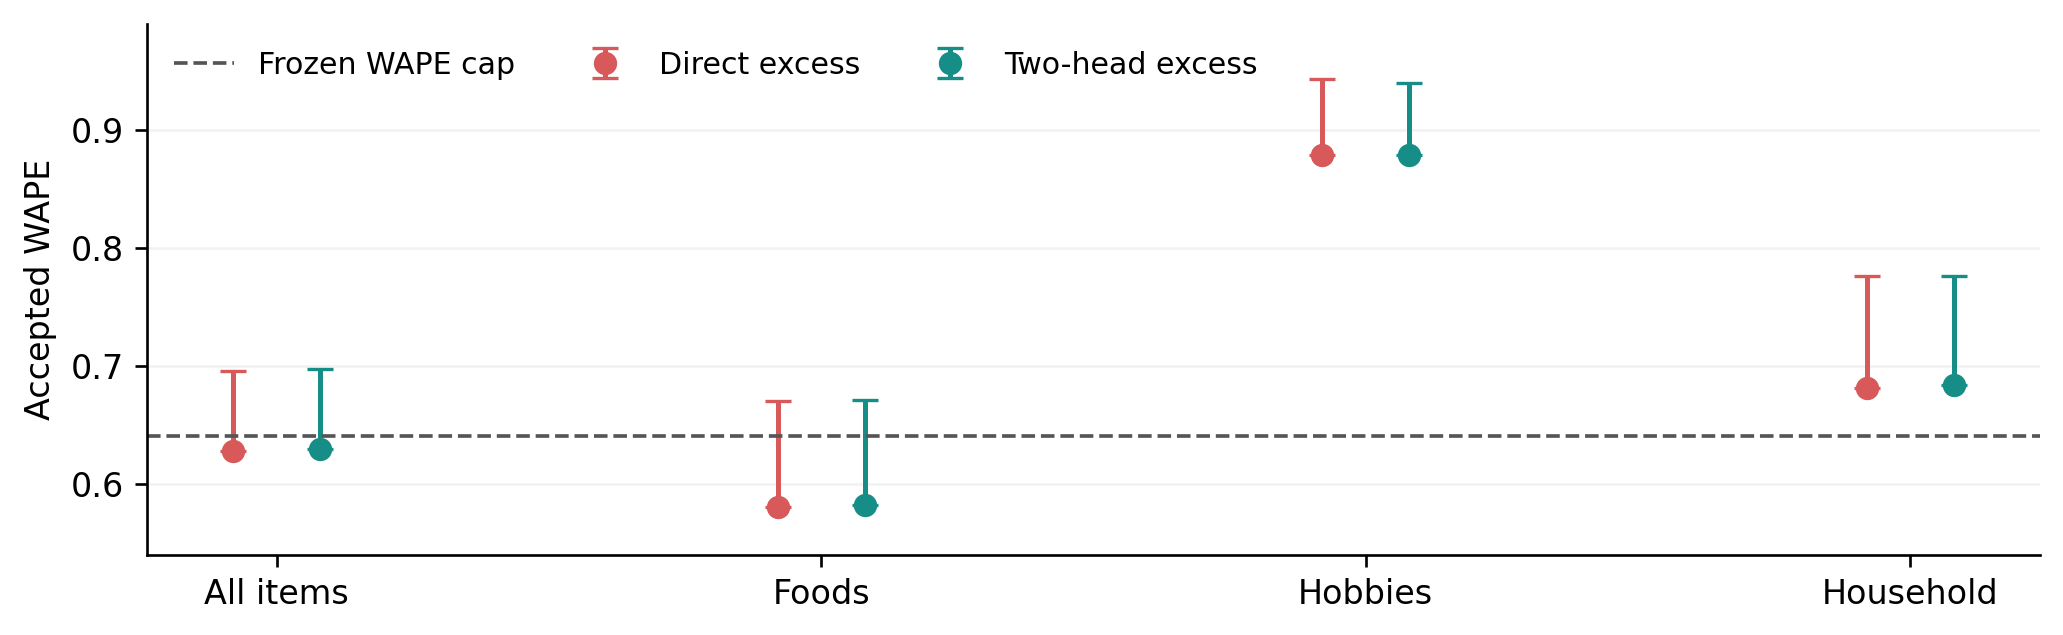
\includegraphics[width=\linewidth]{figures/guardian_groups.png}
\caption{Previously held-out items, first prespecified seed and frozen pooled thresholds. Dots are shadow WAPE; whiskers extend to the one-sided bootstrap upper bound at nominal tail probability $0.05/48$. Hobbies and Household fail the cap even at their point estimates. All displayed adjusted upper bounds exceed the cap.}
\label{fig:guardiangroups}
\end{figure}
\begin{table}[htbp]
\centering\small
\caption{Pooled endpoints from the prespecified first-seed guardian audit. Each bound uses tail probability $0.05/48$ and 10,000 item-bootstrap draws. The full 24-row, 48-endpoint record remains in the supplement; all coverage lower bounds exceed 0.35 and all WAPE upper bounds exceed 0.64013.}
\label{tab:m5guardianbounds}
\begin{tabular}{llrrrr}\toprule
Method & Period & Coverage & WAPE & Cov. lower & WAPE upper\\\midrule
Direct & A & 0.8914 & 0.6399 & 0.8745 & 0.7161\\
Direct & B & 0.8794 & 0.6495 & 0.8630 & 0.7225\\
Direct & Shadow & 0.8725 & 0.6282 & 0.8560 & 0.6959\\
Two-head & A & 0.8895 & 0.6401 & 0.8729 & 0.7160\\
Two-head & B & 0.8763 & 0.6504 & 0.8596 & 0.7236\\
Two-head & Shadow & 0.8746 & 0.6296 & 0.8587 & 0.6971\\
\bottomrule\end{tabular}
\end{table}

Across all four strata, coverage lower bounds range from 0.8040 to 0.9288 and WAPE upper bounds from 0.6704 to 0.9468. Thus every WAPE endpoint misses the cap, including Foods; this is a failure of the specified joint check, not merely the pooled rows in Table~\ref{tab:m5guardianbounds}.
A truncated derived cache was restored from unchanged models; readable arrays matched exactly, and saved masks reproduce all 504 policy/period/stratum records. Frozen results and hashes are unchanged. Subsequent objective, floor, capacity, loss, and partial-label diagnostics reuse this consumed holdout and remain exploratory.

\subsection{The separately frozen external comparison}
\label{app:external}
At 14:29 UTC on 6 September 2026, an initial pending plan froze direct excess versus demand-normalized error with floor 0.25. At 14:47 UTC, after inspecting the consumed first-holdout mixed-utility diagnostics, we replaced that pair with composed excess ($\lambda=1$) versus mixed utility ($\lambda=0.25$). No external data had been accessed under either plan. The earlier plan is preserved byte for byte; the final plan records its hash and replacement reason. The first external access was at 15:10 UTC and evaluation completed at 15:13 UTC. This is a prospectively fixed external comparison selected after first-holdout exploration, not a test independently specified before that exploration.

The final plan fixes 27 dependencies, seed 20260906, the point forecast, 220-tree heads, and development thresholds and scale. No external fit, threshold search, or scale update occurred. Exact values, timestamps, and hash-linked plan history are supplied in the reproduction package.

The 610 external items (269 Foods, 117 Hobbies, 224 Household) yield 140,300 primary rows on days 1919--1941, with every forecast origin after day 1913. Observed history through day 1913 and subsequent observations available at each origin form the features; truth is used only for evaluation. Targets 1914--1918, issued at origin 1911, enter only a prespecified 28-day descriptive sensitivity. Paired item-bootstrap draws (10,000; seed 20260906) test mixed-minus-row demand gain and row loss with one-sided 97.5\% bounds. Both must exclude zero in the specified direction. Separately, two policies, three periods (1919--1941, 1919--1929, 1930--1941), four strata, and two bounds give 48 secondary endpoints, each at tail level $0.05/48$. The primary and secondary families each use nominal 0.05; they do not form one joint 95\% claim. Item resampling retains stores and dates but not shared-shock uncertainty. Because the first holdout failed its operating requirements, this test separately asks whether the fixed coverage contrast transfers and whether the operating constraints hold.

\begin{table}[H]
\centering\small
\caption{One-time external comparison: 610 items, days 1919--1941. Two policies were fixed before opening; thresholds and heads are unchanged. Point WAPE passes the pooled cap, but the 48-endpoint operating check fails.}
\label{tab:external}
\begin{tabular}{lrrr}
\toprule
Fixed policy & Rows (\%) & Demand (\%) & WAPE\\
\midrule
Row utility, $\lambda=1$ & 85.92 & 83.19 & 0.6065 \\
Mixed utility, $\lambda=0.25$ & 82.57 & 88.35 & 0.6081 \\
\bottomrule
\end{tabular}
\par\smallskip\begin{minipage}{0.97\linewidth}\footnotesize
Only the first seed and $\lambda\in\{1,0.25\}$ were frozen for this test. The pair was selected after the first holdout; other external seeds and the full $\lambda$ grid were not evaluated. The test verifies transfer of this selected contrast.
\end{minipage}
\end{table}

\label{sec:external}\label{sec:heldout}
Mixed utility gains 5.16 demand-coverage points and loses 3.35 case points (Table~\ref{tab:external}); both prespecified directional bounds exclude zero. This confirms transfer of the selected contrast, not of the later paired-refit or five-rule menu procedures. Pooled point risks pass, but all 24 adjusted risk upper bounds exceed the cap; all 24 case-coverage lower bounds pass. Hobbies and Household violate the cap at their point estimates. The union remains point-feasible, so this external result establishes neither binding budget competition nor Pareto optimality.

\begin{table}[t]
\centering\small
\caption{All 48 external secondary bounds. Each pair is row-coverage lower bound (\%) / WAPE upper bound; each tail uses $0.05/48$. Every row bound passes 35\%; every WAPE bound fails 0.64013. The two main directional bounds are a separate family.}
\label{tab:external-bounds}
\begin{tabular}{llrr}
\toprule
Period & Stratum & $\lambda=1$ & $\lambda=0.25$\\
\midrule
All 23 days & All & 83.90 / 0.6896 & 80.81 / 0.6863 \\
 & Foods & 78.70 / 0.6634 & 76.73 / 0.6684 \\
 & Hobbies & 75.58 / 0.9171 & 76.99 / 0.8864 \\
 & Household & 91.57 / 0.7813 & 84.64 / 0.7618 \\
First 11 days & All & 83.10 / 0.6908 & 80.56 / 0.6896 \\
 & Foods & 77.30 / 0.6637 & 76.12 / 0.6727 \\
 & Hobbies & 75.72 / 0.9161 & 77.02 / 0.8803 \\
 & Household & 90.98 / 0.7824 & 84.51 / 0.7642 \\
Last 12 days & All & 84.48 / 0.6907 & 81.00 / 0.6860 \\
 & Foods & 79.78 / 0.6658 & 77.08 / 0.6643 \\
 & Hobbies & 75.55 / 0.9201 & 76.84 / 0.8937 \\
 & Household & 91.99 / 0.7791 & 84.62 / 0.7637 \\
\bottomrule
\end{tabular}
\end{table}

The full-28-day sensitivity has row/demand coverage 86.14\%/82.87\% for $\lambda=1$ and 82.51\%/87.94\% for $\lambda=0.25$, with WAPE 0.6128/0.6133. It is descriptive only. The archived execution has one opening, zero fits, and zero threshold searches; saved item-level accepted counts, error sums, and demand sums reproduce the primary bounds and all 48 secondary endpoints.

\paragraph{Descriptive external budget accounting.}
We apply equation~\eqref{eq:budget} retrospectively to the same saved masks (Table~\ref{tab:externalbudget}). Row-only and mixed-only sets spend 30.20\% and 29.45\% of common slack, yet contain 3.32\% and 8.48\% of demand. Both retain slack; the joint operating failure remains. This adds no confirmatory endpoint, fit, threshold, or policy; the superseded pair is not evaluated.
\begin{table}[t]
\centering\small
\caption{Descriptive budget accounting for the two frozen external policies, days 1919--1941. $K$ is their intersection; $U$ is accepted only at $\lambda=1$, and $V$ only at $\lambda=0.25$. Demand shares use the total 209,893 units. Signed excess is $E_B-rM_B$; a negative value supplies slack. This analysis reuses saved predictions after the confirmation result.}
\label{tab:externalbudget}
\begin{tabular}{lrrrrr}
\toprule
Set & Rows & Demand (\%) & WAPE & Mean $f$ & Excess \\
\midrule
Common $K$ & 109,985 & 79.86 & 0.5899 & 1.112 & -8,421.10 \\
Row-only $U$ & 10,557 & 3.32 & 1.0046 & 0.122 & 2,542.83 \\
Mixed-only $V$ & 5,855 & 8.48 & 0.7794 & 1.703 & 2,480.43 \\
\bottomrule
\end{tabular}
\end{table}


\subsection{Retained historical controls and reproduction}
\label{app:history}\label{app:legacyselection}
The numerical supplement retains the earlier weak-forecast controls and all seed/category/period reports. The prior FreshRetailNet check used observable evaluation labels, not hidden stockout demand: shadow row coverage/WAPE 0.28163/0.30484 missed both 0.30 targets, with adjusted bounds 0.25713/0.31821. Calibration B's coverage lower bound was 0.28498. This failed check supplies no natural-stockout confirmation.

The notebook checks frozen hashes before and after replaying theory, moments, and external sufficient statistics. All verification output goes to a separate directory. Experiment scripts regenerate fits from public M5. The separate numerical assets include the derived development inputs needed for the new predictor-specific selector replay; original external replay uses retained sufficient statistics.

\section{Objective choice and supervised-head diagnostics}
\label{app:objective}
\begin{table}[t]
\centering\small
\caption{Strong fixed forecaster; three matched risk-training seeds. Values are development-shadow means $\pm$ training-seed SD (not independent-test uncertainty). Thresholds use the same two calibration blocks and row-coverage objective. Numbers in parentheses denote total boosting trees. The two-head budget-220 control uses 110 trees per head.}
\label{tab:twohead}
\begin{tabular}{lrrr}\toprule
Score & Row coverage (\%) & Demand coverage (\%) & WAPE\\\midrule
Forecast-normalized & 80.22 $\pm$ 0.27 & 86.58 $\pm$ 0.09 & 0.6216 \\
Demand-normalized & 74.17 $\pm$ 0.85 & 89.01 $\pm$ 0.20 & 0.6260 \\
Forecast excess & 81.47 $\pm$ 0.41 & 70.71 $\pm$ 0.59 & 0.6222 \\
Two-head excess (440) & 86.35 $\pm$ 0.08 & 81.32 $\pm$ 0.21 & 0.6268 \\
Two-head excess (220) & 86.61 $\pm$ 0.12 & 81.88 $\pm$ 0.29 & 0.6269 \\
Direct excess (220) & 86.30 $\pm$ 0.16 & 80.86 $\pm$ 0.11 & 0.6245 \\
\bottomrule\end{tabular}
\end{table}

\begin{table}[t]
\centering\small
\caption{Explicit objective-based family selection among the seven original scores, followed by threshold application to shadow periods. Three-seed means. Both objectives retain WAPE cap 0.64013 and row floor 0.35 in calibration A/B. Guardian rows are post-hoc reuse of the same consumed holdout, not new confirmation.}
\label{tab:objectives}
\begin{tabular}{lllrrr}\toprule
Cohort & Objective & Selected score & Rows (\%) & Demand (\%) & WAPE\\\midrule
Design & Row & Direct excess (220) & 86.30 & 80.86 & 0.6245 \\
Guardian & Row & Direct excess (220) & 87.37 & 83.29 & 0.6280 \\
Design & Demand & Demand-normalized & 74.17 & 89.01 & 0.6260 \\
Guardian & Demand & Demand-normalized & 73.62 & 88.23 & 0.6219 \\
\bottomrule\end{tabular}
\end{table}

\subsection{Architecture controls and first-holdout detail}
\label{app:architecture}
\paragraph{Development accepted-set accounting.}
Direct excess gains 6.08 percentage points in mean row coverage over forecast-normalized error, but loses 5.71 points of demand coverage. At the first seed, their common accepted set covers 73.35\% of rows and has WAPE 0.5958, leaving slack under the 0.64013 cap. The direct-only set adds 267,656 rows (12.84\% of all rows), but only 5.69\% of demand; its WAPE is 1.0026. The relative-only set contains 141,617 rows and 11.45\% of demand, with WAPE 0.7915. Mean forecasts in the two differing sets are 0.039 and 1.498 units. In equation~\eqref{eq:budget}, the common set supplies 97,185.97 units of excess slack. The direct-only set consumes 60,141.11 (61.88\%), versus 50,549.56 (52.01\%) for the relative-only set. Both fit within the pooled budget despite their individual WAPE exceeding the cap. This accounts for the row gain through budget use and demand composition.


\paragraph{Architecture is distinct from acceptance utility.}
The original matched selector comparison provides an architectural control. Direct-excess, two-head, and matched-tree-budget two-head scores reach 86.30\%, 86.35\%, and 86.61\% mean row coverage. Direct learning has slightly lower accepted WAPE (0.6245 versus 0.6268 and 0.6269); it does not establish a direct-learning advantage. The informative distinction is the coverage objective and resulting budget allocation, not whether excess is learned directly or composed from two heads. Full three-seed results are in Appendix~\ref{app:objective}.

\subsection{Detailed first item-holdout comparison}
\label{app:architecture-holdout}
\begin{table}[t]
\centering\small
\caption{Previously held-out M5 items: fixed pooled thresholds, 610 items, 6,100 series, and 695,400 shadow rows. Three-seed means; all fits and thresholds were frozen before opening. Seeds measure training variability, not three independent holdouts. Absolute-error selection accepts no rows and has undefined WAPE.}
\label{tab:m5guardian}
\begin{tabular}{lrrr}\toprule
Score & Row coverage (\%) & Demand coverage (\%) & WAPE\\\midrule
Forecast-normalized & 80.87 & 87.65 & 0.6219 \\
Demand-normalized & 73.62 & 88.23 & 0.6219 \\
Forecast excess & 82.74 & 74.59 & 0.6251 \\
Two-head excess (440) & 87.41 & 83.69 & 0.6297 \\
Two-head excess (220) & 87.67 & 84.18 & 0.6297 \\
Direct excess (220) & 87.37 & 83.29 & 0.6280 \\
\bottomrule\end{tabular}
\end{table}

The freeze specifies seven scores, two threshold modes, three seeds, and a first-seed direct-versus-two-head primary contrast. The holdout uses the same A/B and later evaluation dates, without recalibration; no holdout outcome selects an original policy. Its shadow contains 695,400 rows on days 1800--1913.

The coverage trade-off persists (Table~\ref{tab:m5guardian}). Across three fixed fits, direct excess increases row coverage by 6.49 percentage points over forecast-normalized error while reducing demand coverage by 4.36 points. Two-head coverage is 87.41\%, compared with 87.37\% for direct learning, with WAPE 0.6297 versus 0.6280. At the prespecified first seed, direct minus two-head row coverage is $-0.215$ points (paired 95\% item-bootstrap interval $[-0.413,-0.018]$ points); direct WAPE is lower by 0.00141. These are different trade-offs, not an equivalence result or a direct-learning advantage.



Operating constraints do not transfer jointly. First-seed direct and two-head shadow WAPE are 0.6282 and 0.6296 pooled, but approximately 0.879 for Hobbies and 0.682--0.683 for Household. In the holdout window matching calibration B, even pooled WAPE is 0.6495 and 0.6504, above the 0.64013 cap. All frozen category-specific policies abstain entirely on Hobbies because their development threshold is absent. The prespecified 48-endpoint family covers two primary methods, three periods, four strata, and two bounds, using 10,000 item-bootstrap draws. Every coverage lower bound exceeds 0.35, but every adjusted WAPE upper bound exceeds the cap; shadow pooled upper bounds are 0.6959 and 0.6971. This fails the specified joint operating check. Appendix~\ref{app:heldout} reports all bounds and the access record.


\begin{figure}[t]
\centering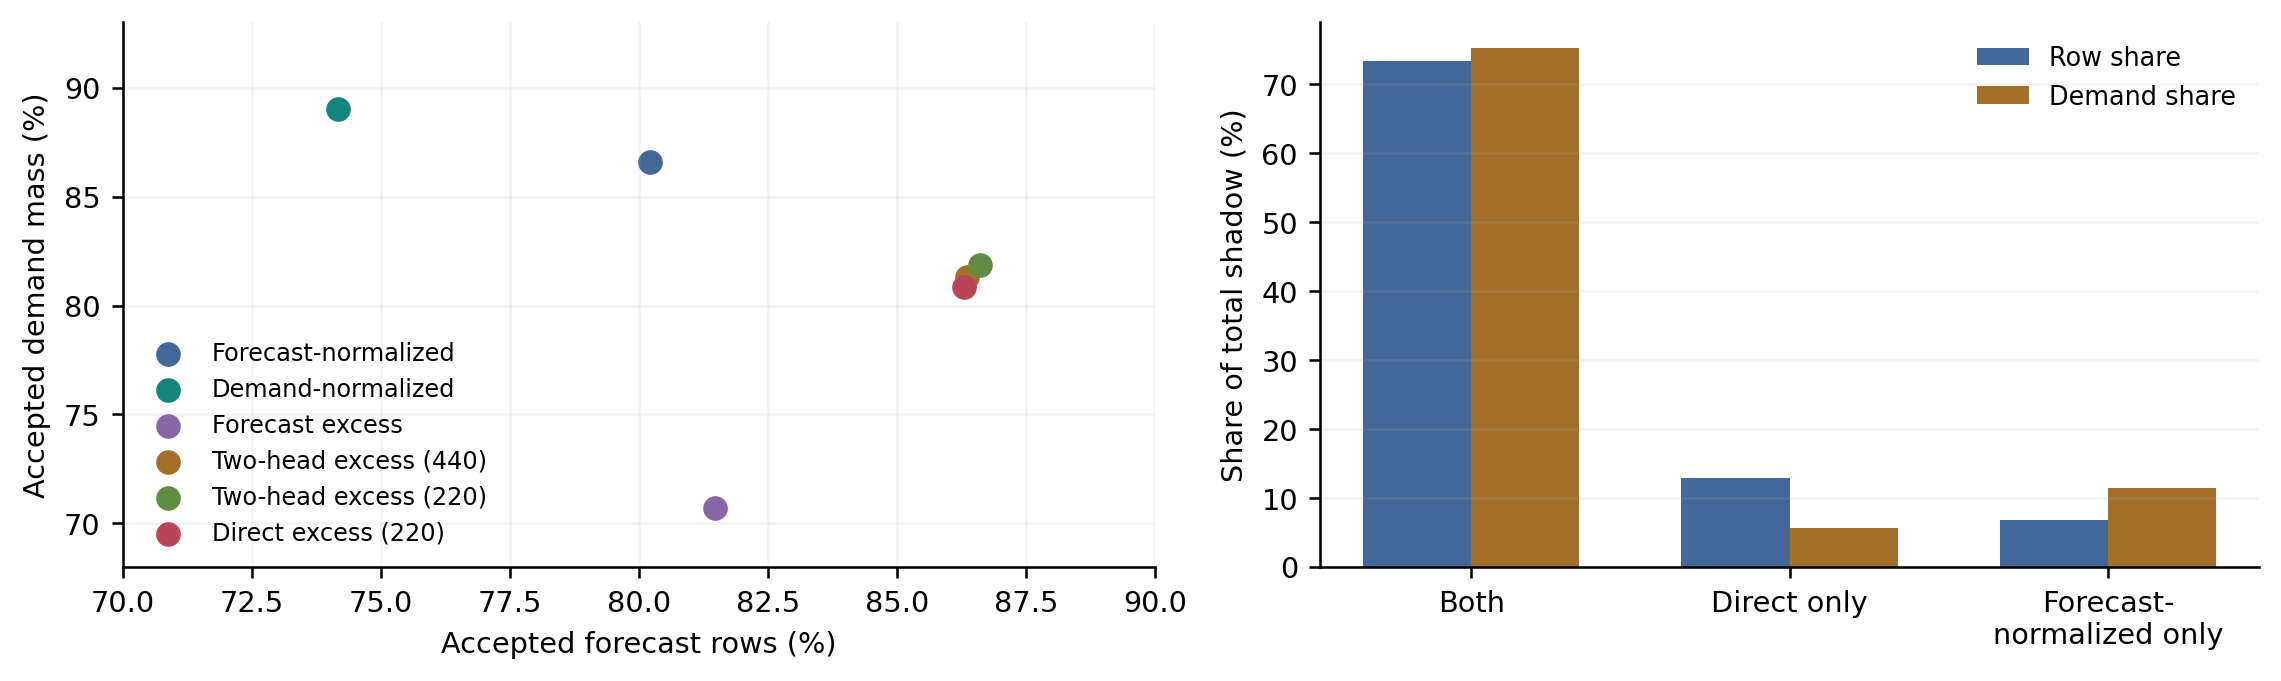
\includegraphics[width=\linewidth]{figures/row_vs_demand.png}
\caption{Original development comparison. Left: three-seed means under row-coverage threshold selection. Right: first-seed direct-excess and forecast-normalized-error acceptance sets. The direct-only set has more cases and less demand. These previously evaluated results precede the additional menu audit.}
\label{fig:mass}
\end{figure}


\subsection{Nested paths, family choice, and denominator regularization}
For a fixed score, $A_t=\{s\leq t\}$ is nested. Both $P(A_t)$ and $\E[Y\ind_{A_t}]/\E Y$, including their empirical blockwise minima, are nondecreasing in $t$. WAPE need not be monotone, but the largest member of any nonempty finite feasible grid maximizes either coverage. An empty grid returns no policy.

Across 27 score/seed pairs (nine rankings, three fits), changing only the coverage objective leaves all thresholds unchanged: 24 finite and three infeasible. Family choice instead selects direct excess for rows and demand normalization for demand. The later audit uses the largest maximizer, changing 1--3 shadow rows in four configurations relative to the original first-maximizer convention; frozen results are preserved.

\texttt{CAP\_REFERENCE.json} reproduces the legacy development-selection WAPE 0.7530939208313988 and the archived cap $r=.85\times.7530939208313988$. Table~\ref{tab:floors} varies the unit-sales denominator regularizer without guardian-based selection. Demand normalization wins the family comparison at floor 0.25; the smaller-floor reversals limit any claim about estimated $e/\mu$.
\begin{table}[htbp]
\centering\small
\caption{First-seed denominator-floor sensitivity on consumed guardian shadow. F/D denote forecast/demand normalization. Thresholds use development A/B; no floor is selected on guardian. Full development metrics remain in the numerical supplement.}
\label{tab:floors}
\begin{tabular}{rrrrr}\toprule
Floor & F demand (\%) & D demand (\%) & F WAPE & D WAPE\\\midrule
0 & 87.77 & 87.53 & 0.6195 & 0.6186\\
0.01 & 87.75 & 87.53 & 0.6193 & 0.6186\\
0.05 & 87.97 & 87.53 & 0.6201 & 0.6186\\
0.1 & 87.98 & 87.58 & 0.6206 & 0.6188\\
0.25 & 87.73 & 88.10 & 0.6219 & 0.6211\\
0.5 & 85.53 & 89.11 & 0.6249 & 0.6257\\
1 & 74.47 & 86.32 & 0.6286 & 0.6297\\
\bottomrule\end{tabular}
\end{table}


\subsection{Mixed utility and the zero-floor comparison}
\label{app:mixed}
For a nonbinding row floor, $w_\lambda=\lambda+(1-\lambda)\mu/T$ defines a probability measure since $\E w_\lambda=1$. At fixed $U_\lambda=\E[aw_\lambda]$, the exchange proof orders $m_r/w_\lambda$ and minimizes excess. Largest feasible weighted prefixes maximize that utility; boundary randomization handles ties. At $\lambda=0$, reject $\mu=0,e>0$ without losing utility; zero-error/zero-demand contexts are neutral. With a binding row floor, a finite-policy LP has Lagrangian coefficient $w_\lambda+\zeta-\tau m_r$, $\zeta\geq0$. If $\tau>0$, its score is $m_r/(w_\lambda+\zeta)$, with $\zeta(c-c_0)=0$. Thus the simple score alone need not solve a binding-floor problem.

The exploratory grid uses first-seed 220-tree heads, zero-clipping, and development A/B mean demand $\hat T$. A/B outcomes alone select thresholds. All five guardian policies are reported; each fails period-B pooled WAPE. At $\lambda=0$, positive-error/zero-demand rows rank last and $0/0$ is zero. The mixed $\lambda=0.25$ point exceeds $\lambda=0$ in both coverages; imperfect fitted heads permit this empirical dominance.
\begin{table}[htbp]\centering\small
\caption{Fixed mixed-utility grid on consumed guardian predictions (one predeclared fit). All choices are made on development A/B; no guardian-best mixture is selected.}
\label{tab:mixed}
\begin{tabular}{rrrrr}\toprule
$\lambda$ & Shadow rows (\%) & Shadow demand (\%) & Shadow WAPE & B WAPE\\\midrule
0 & 62.74 & 87.53 & 0.6186 & 0.6428\\
0.25 & 84.31 & 88.67 & 0.6272 & 0.6467\\
0.5 & 86.42 & 87.87 & 0.6287 & 0.6473\\
0.75 & 87.28 & 86.24 & 0.6292 & 0.6488\\
1 & 87.46 & 83.78 & 0.6296 & 0.6504\\
\bottomrule\end{tabular}\end{table}

\begin{table}[htbp]
\centering\small\setlength{\tabcolsep}{3.2pt}
\caption{Development mixed-utility path before item transfer. One common A/B-selected threshold per $\lambda$; first-seed heads. Coverages are percentages. All A/B pooled point constraints pass; these reused calibration outcomes give no independent risk guarantee.}
\label{tab:mixed-development}
\begin{tabular}{r rrr rrr rrr}\toprule
&\multicolumn{3}{c}{Calibration A}&\multicolumn{3}{c}{Calibration B}&\multicolumn{3}{c}{Later evaluation}\\
$\lambda$&Rows&Demand&WAPE&Rows&Demand&WAPE&Rows&Demand&WAPE\\\midrule
0 & 71.68 & 89.85 & 0.6401 & 67.45 & 88.45 & 0.6381 & 64.22 & 88.43 & 0.6231\\
0.25 & 85.25 & 88.67 & 0.6396 & 84.06 & 87.97 & 0.6401 & 83.77 & 88.54 & 0.6278\\
0.5 & 86.71 & 86.91 & 0.6388 & 85.69 & 86.57 & 0.6401 & 85.63 & 87.02 & 0.6278\\
0.75 & 87.54 & 84.68 & 0.6387 & 86.46 & 84.45 & 0.6401 & 86.36 & 84.68 & 0.6277\\
1 & 87.83 & 81.56 & 0.6390 & 86.63 & 81.46 & 0.6401 & 86.42 & 81.56 & 0.6275\\
\bottomrule\end{tabular}
\end{table}

Without a positive floor, forecast-normalized guardian row/demand coverage is 44.62\%/87.77\% (WAPE 0.6195), versus demand-normalized 62.74\%/87.53\% (0.6186). The latter masks equal the $\lambda=0$ endpoint, as required by their affine score relationship.

\subsection{Error-head bottleneck and finite-capacity effects}
\begin{table}[htbp]
\centering\small
\caption{Hobbies outcome substitutions, first seed. Each path optimizes its own later-window threshold, using realized labels in the excess score. Coverages are percentages; dashes mean no feasible prefix. These are samplewise diagnostics, not deployable conditional-mean oracles.}
\label{tab:partialoracles}
\begin{tabular}{lrrr rrr}\toprule
&\multicolumn{3}{c}{Development}&\multicolumn{3}{c}{Item holdout}\\
Replaced head&Rows&Demand&WAPE&Rows&Demand&WAPE\\\midrule
Neither&0.00&0.00&--&0.00&0.00&--\\
Error only&76.78&23.90&0.6401&76.38&21.28&0.6401\\
Demand only&0.00&0.00&--&0.00&0.00&--\\
Both&89.15&60.94&0.6401&86.97&54.04&0.6401\\
\bottomrule\end{tabular}
\end{table}

The outcome-substitution diagnostic (Table~\ref{tab:partialoracles}) localizes a samplewise error-information gap. Positive-error/zero-demand rows rank last; zero-error/zero-demand rows cost no excess. Realized-label access includes irreducible noise and is not a conditional-learning guarantee.

Three 220-tree error-head interventions hold the point forecast and demand head fixed. Two Hobbies specialists share 107,384 rows from the original sample; their 21-versus-29-feature contrast holds the training population fixed. A new shared 29-feature head uses exactly the original 600,000 rows, resolving sample-size confounding for feature addition relative to the shared 21-feature head. Added features are positive-day count, positive-size mean/CV$^2$, and recency over 56/112 days ending at the origin. Protocols precede fitting; shared sample indices, the Hobbies subset, and original forecasts reproduce bit for bit. Future perturbations leave features unchanged. The shared 29-feature head improves both reported MSEs but yields no feasible A/B threshold or later-block prefix (Table~\ref{tab:hobbies_intervention}). Training still uses pre-censoring error labels; no new head is evaluated on either holdout. No matched Hobbies point-forecast intervention is available, so attribution to the point model remains unresolved.
\begin{table}[t]
\caption{Development Hobbies interventions, first seed. The two shared heads use the same 600,000 rows; the two specialists use the same 107,384 Hobbies rows. All use 220 trees, the same point forecast and demand head. MSE uses the later development block. No common A/B threshold, or outcome-informed later-block prefix, meets the cap and 35\% row floor. Empty-policy WAPE is undefined.}
\label{tab:hobbies_intervention}
\centering
\small
\setlength{\tabcolsep}{3pt}
\begin{tabular}{lrrrrrr}
\toprule
Error head & Train rows & MSE & Positive MSE & Rows (\%) & WAPE & Prefix (\%) \\
\midrule
Shared, 21 features & 600,000 & 2.3554 & 7.8403 & 0.00 & -- & 0.00 \\
Shared, 29 features & 600,000 & 2.3370 & 7.7650 & 0.00 & -- & 0.00 \\
Hobbies, 21 features & 107,384 & 2.4232 & 7.9048 & 0.00 & -- & 0.00 \\
Hobbies, 29 features & 107,384 & 2.4399 & 7.9392 & 0.00 & -- & 0.00 \\
\bottomrule
\end{tabular}
\end{table}

Capacity controls show that enlarging only the error head lowers held-out row coverage by 0.45--0.63 points, whereas enlarging only demand raises it by 0.20--0.38 points and raises WAPE. Both heads together increase excess MSE from 1.0630 to 1.0868. The numerical supplement retains all 288 error/demand/cross-moment decompositions.

\subsection{Demand-head loss controls}
Squared, Poisson, and Tweedie losses target the conditional mean under their respective moment assumptions; the supplement gives the derivatives. Six matched 220-tree Poisson/Tweedie ($p=1.5$) demand heads improve held-out demand coverage, but period-B WAPE remains 0.6470/0.6467. Full seed results are archived.

\subsection{Group-budget control in a fixed learned-score class}
\label{app:grouplp}
For each category, predicted error and demand from the first-seed 220-tree heads define an $8\times8$ quantile grid using development A/B scores only. Bin probabilities $z_j\in[0,1]$ are shared across both blocks. The LP maximizes minimum block row coverage, enforcing $\sum_j z_j(E_{gjb}-rM_{gjb})\leq0$ and $\sum_jz_jN_{gjb}\geq0.35N_{gb}$ separately for each group $g$ and block $b$. No category borrows another's budget. Calibration outcomes determine the probabilities; bins, coefficients, and probabilities are fixed before application to the consumed guardian. These are exploratory point constraints, not independent calibration bounds.

All 28 occupied Hobbies bins in A and 29 in B have positive excess. Their minimum WAPE is 0.7289866 and 0.7503685, respectively, so every nonempty fractional mixture has WAPE above the cap in either block. At the row floor, a dual certificate bounds the minimum worst-block mean excess below by 0.0142589987 units per original row. The supplement supplies coefficients and a verifier checking residual-corrected dual bounds. This infeasibility concerns the specified grid, not arbitrary features or acceptance rules.

Foods and Household attain minimum calibration row coverage 94.60\% and 76.76\%. Their transferred guardian B WAPE is 0.6392 and 0.6459; shadow WAPE is 0.6111 and 0.6455. Thus the group constraints expose Hobbies failure and retain Household transfer failure. Fractional metrics are ratios of expected accepted sums; a realized randomized deployment can fluctuate around them.

\section{Observed-sales and capacity likelihood controls}
\label{app:observable}
\begin{table}[t]
\centering\small\setlength{\tabcolsep}{3pt}
\caption{First-seed NB grid on development data. A/B/shadow pairs are implied / realized WAPE; rows are shadow coverage. The star selects observed validation NLL among $\{1,1.5,2,3,5\}$; 0.5/10 are descriptive anchors. Intervals are $10^{-3}$ NLL differences from shape 2, with four-comparison Bonferroni adjustment using 10,000 paired item-bootstrap draws. They reuse the selection data and condition on fitted models. Dashes in risk columns mean no admissible threshold.}
\label{tab:nb-fine-grid}
\begin{tabular}{rrrrrrr}
\toprule
$\kappa$ & Valid. NLL & $\Delta$NLL interval & Calibration A & Calibration B & Shadow & Rows (\%)\\
\midrule
0.5 & 0.7541 & -- & -- / -- & -- / -- & -- / -- & 0.00 \\
1 & 0.7361 & [2.934, 6.334] & -- / -- & -- / -- & -- / -- & 0.00 \\
1.5 & 0.7324 & [0.220, 1.634] & -- / -- & -- / -- & -- / -- & 0.00 \\
2 * & 0.7314 & reference & 0.6401 / 0.5597 & 0.6376 / 0.5578 & 0.6365 / 0.5484 & 48.74 \\
3 & 0.7322 & [-0.008, 1.592] & 0.6401 / 0.6421 & 0.6368 / 0.6412 & 0.6355 / 0.6311 & 79.48 \\
5 & 0.7347 & [1.606, 5.031] & 0.6401 / 0.6861 & 0.6361 / 0.6856 & 0.6334 / 0.6748 & 99.41 \\
10 & 0.7392 & -- & 0.6076 / 0.6902 & 0.6033 / 0.6888 & 0.5997 / 0.6790 & 100.00 \\
\bottomrule
\end{tabular}
\end{table}

\subsection{Observation model and available information}
This development-only experiment keeps the plain observed-sales L1 forecast fixed; forecast choice and the cap inherit outcome-informed development history. The strict benchmark flag $\Delta=\ind\{Y>C\}$ differs from the observable capacity hit $H=\ind\{S\geq C\}$, which reveals only $Y\geq C$. The capacity branch uses $H$ in both responses and historical features. Each fit samples 600,000 risk rows from days 1436--1532, validates on 1534--1553, and uses 34 origin-valid inputs, 220 trees, 31 leaves, and the common training settings. Three seeds are retained; shape selection uses observed-data validation likelihood.

Let $p_\theta(y\mid X)$ be Poisson with mean $\mu_\theta$, or NB with mean $\mu_\theta$ and fixed shape $\kappa$ (variance $\mu_\theta+\mu_\theta^2/\kappa$). The two negative log likelihoods are
\begin{align*}
 \ell_\Delta&=-(1-\Delta)\log p_\theta(S\mid X)-\Delta\log\Pr_\theta(Y>C\mid X),\\
 \ell_H&=-(1-H)\log p_\theta(S\mid X)-H\log\Pr_\theta(Y\geq C\mid X).
\end{align*}
For integer counts, the latter survival is evaluated at $C-1$. These likelihoods require an appropriate conditional count family and ignorable censoring given modeled information. Dependence of capacity on past sales does not automatically justify ignorability for a finite feature vector. The method therefore models the hidden tail; it does not nonparametrically identify it.

\subsection{Implied moments, thresholding, and results}
For $k=\lfloor f\rfloor$ and nonnegative $f$, the distribution implies
\[
 \hat e=\E_\theta|Y-f|=\hat\mu-f+2\{fF_\theta(k)-\E_\theta[Y\ind\{Y\leq k\}]\}.
\]
The truncated moment is $\hat\mu F_{\operatorname{Pois}(\hat\mu)}(k-1)$ for Poisson and $\hat\mu F_{\operatorname{NB}(\kappa+1,p)}(k-1)$ for NB, with $p=\kappa/(\kappa+\hat\mu)$. Direct summation and finite differences check moments and likelihood derivatives, including extreme tails.

A/B thresholds maximize common row coverage under $\sum a\hat e/\sum a\hat\mu\leq r$ and the 0.35 floor. Both excess and demand-normalized rankings are archived. Implied and realized risk differ through
\[
 R(a)-r=\frac{\E[a(\hat e-r\hat\mu)]+\E[a(e-\hat e)]-r\E[a(\mu-\hat\mu)]}{\E[a\mu]}.
\]
Hence passing the implied constraint is not an observed-risk certificate. Table~\ref{tab:observablemoments} reports both numerator/denominator pairs.

\begin{table}[t]
\centering\small
\caption{Sales-and-capacity NB $\kappa=2$ at its observed-likelihood-selected, model-implied threshold. Bias is $(\widehat E/E-1)$ or $(\widehat M/M-1)$ on the same accepted rows. Each entry averages three fit-specific ratios. Positive error-mass bias exceeds positive demand-mass bias, making the implied ratio conservative in aggregate.}
\label{tab:observablemoments}
\begin{tabular}{lrrrrr}
\toprule
Period & Rows (\%) & Implied WAPE & Realized WAPE & Error bias (\%) & Demand bias (\%)\\
\midrule
A & 49.96 & 0.6401 & 0.5568 & +18.82 & +3.35\\
B & 49.44 & 0.6376 & 0.5562 & +21.65 & +6.12\\
Shadow & 48.17 & 0.6365 & 0.5461 & +20.59 & +3.46\\
\bottomrule\end{tabular}\end{table}

Across three fits per observation branch, validation selects $\kappa=2$; Hobbies WAPE remains 0.8018. All 33 retained fits and seven derivative, moment, origin, and equality tests are archived.

\FloatBarrier
\subsection{Fine dispersion grid and identical-forecast comparison}
All fine-grid fits share the sample, features, and forecast; protocols and hashes precede fitting. The count-matched supervised head uses the same inputs and a realized-excess target. Outcome-independent boundary draws agree with fractional-tie expectations (264 records and 21 count matches verified). Uniform fractional abstention at 48.17\% instead has equal demand coverage and WAPE 0.6790.

\paragraph{Validation likelihood uncertainty.}
All seven observed NLL means reproduce exactly. The 10,000 paired-bootstrap draws resample 1,829 validation items (365,800 rows), retaining each item's stores and dates. The four adjusted comparisons use two-sided tails $0.05/(2\times4)$; pointwise 95\% intervals are all positive. These approximate intervals reuse the data that selected shape 2 and condition on fitted models; they neither confirm the selected winner independently nor identify censored tails. Shared store/calendar shocks remain unaccounted for. Saved item sums reproduce all intervals without fitting.

\subsection{Observed-data diagnostics and their target population}
\label{app:natural-diagnostics}
Theoretical selection uses conditional loss and exposure; naturally hidden demand does not supply either without assumptions. Our observed-sales-and-capacity negative-binomial experiment illustrates the issue. Among adjusted paired item-bootstrap comparisons, shape $\kappa=3$ is the only candidate whose validation likelihood difference from selected $\kappa=2$ includes zero, yet it breaks both realized calibration caps that $\kappa=2$ passes. The selected model overestimates aggregate error mass by 20.59\%; its pooled point pass does not validate conditional moments. Appendix~\ref{app:observable} provides the likelihood, dispersion grid, and count-matched supervised control.

Further forecasting experiments on naturally stockout-annotated FreshRetailNet test observable sales outcomes, not hidden demand. A forward-time residual learner reduces WAPE on the 8,020 non-stockout test rows from 0.32928 to 0.29201, and on all 14,000 recorded-sales rows from 0.36162 to 0.33401. These later comparisons reuse the previously opened seven-day cohort; most improvement remains without the risk feature (non-stockout WAPE 0.29289). They demonstrate useful forecast adaptation within that evaluated population, but cannot certify an acceptance constraint for demand coverage on unobserved stockout demand. Appendix~\ref{app:accuracy} records the controls and uncertainty. Thus accuracy improvement, acceptance utility, and identification are three distinct requirements of a forecasting engine.


